% 来源：固定候选 PDF，山东文科，PDF 第1页（印刷页322），Q3 四选项。
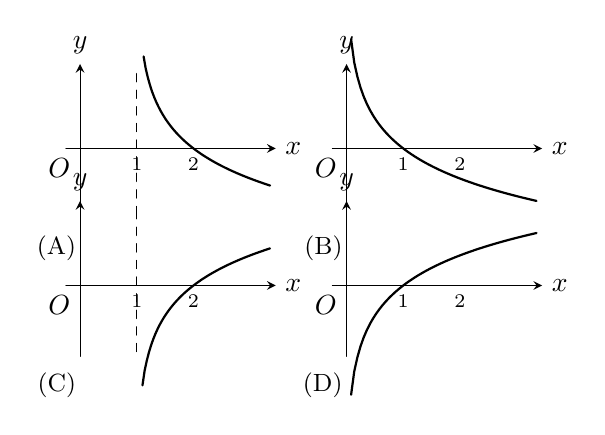
\begin{tikzpicture}[x=0.72cm,y=0.58cm,>=stealth,line cap=round,line join=round]
\tikzset{axis/.style={->,thin},curve/.style={thick},asym/.style={dashed,thin}}
\foreach \x/\y/\idx/\lbl in {0/3/0/A,4.7/3/1/B,0/0/2/C,4.7/0/3/D}{
  \begin{scope}[shift={(\x,\y)}]
    \draw[axis] (-0.25,0)--(3.45,0) node[right] {$x$};
    \draw[axis] (0,-1.55)--(0,1.85) node[above] {$y$};
    \node[below left] at (0,0) {$O$};
    \node[below] at (1,0) {\scriptsize 1};
    \node[below] at (2,0) {\scriptsize 2};
    \node[below left] at (0.1,-1.7) {\small (\lbl)};
    \ifcase\idx
      \draw[asym] (1,-1.45)--(1,1.7);
      \draw[curve,domain=1.12:3.35,samples=60] plot (\x,{ -0.95*ln(\x-1) });
    \or
      \draw[curve,domain=0.08:3.35,samples=60] plot (\x,{ -0.95*ln(\x) });
    \or
      \draw[asym] (1,-1.45)--(1,1.7);
      \draw[curve,domain=1.1:3.35,samples=60] plot (\x,{ 0.95*ln(\x-1) });
    \or
      \draw[curve,domain=0.08:3.35,samples=60] plot (\x,{ 0.95*ln(\x) });
    \fi
  \end{scope}
}
\end{tikzpicture}
